\documentclass[10pt]{beamer}

\usetheme{CambridgeUS}
\usepackage[english, russian]{babel}
\usepackage[utf8]{inputenc}
\usepackage{caption}
\usepackage{etoolbox}
\usepackage{multicol}
\usepackage{movie15}

\title[\href{https://goo.gl/NRgp8K}{https://goo.gl/NRgp8K} (Term 3)]{Диаграмы Вороного}
\author[Гусев Илья]{Гусев Илья}
\institute[МФТИ] 
{Московский физико-технический институт\\*}
\date{Москва, 2018}
\subject{Computer Science}

\begin{document}

\begin{frame}
  \titlepage
\end{frame}

\begin{frame}{Содержание}
\tableofcontents
\end{frame}

\section{Диаграммы Вороного}
\subsection{Что это?}
\begin{frame}[fragile]{Что это?}
\begin{center}
    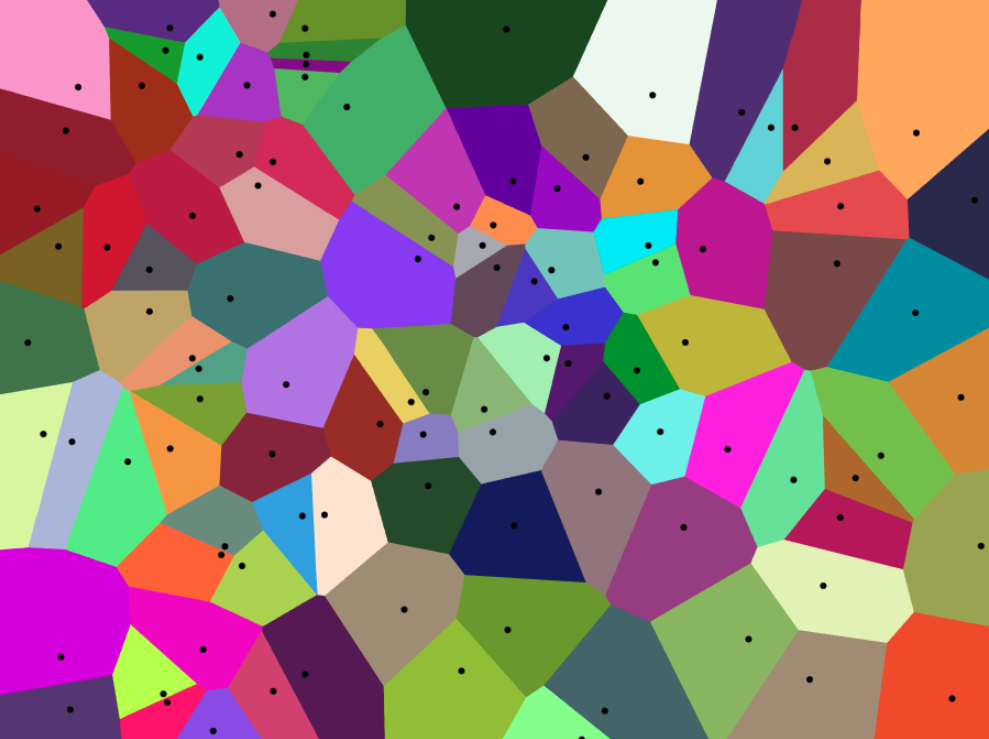
\includegraphics[width=10cm, height=7.2cm]{Term_3/Source/Pictures/voronoi_example.png}
\end{center}
\end{frame}

\subsection{Варианты построения}
\begin{frame}[fragile]{Варианты построения}
\begin{enumerate}
    \item Навиный алгоритм
    \item Модификации навиного алгоритма
    \item Алгоритм Форчуна (sweep line)
    \item Резделяй и властвуй
\end{enumerate}
\end{frame}

\subsection{Наивный алгоритм}
\begin{frame}[fragile]{Наивный алгоритм}
\begin{center}
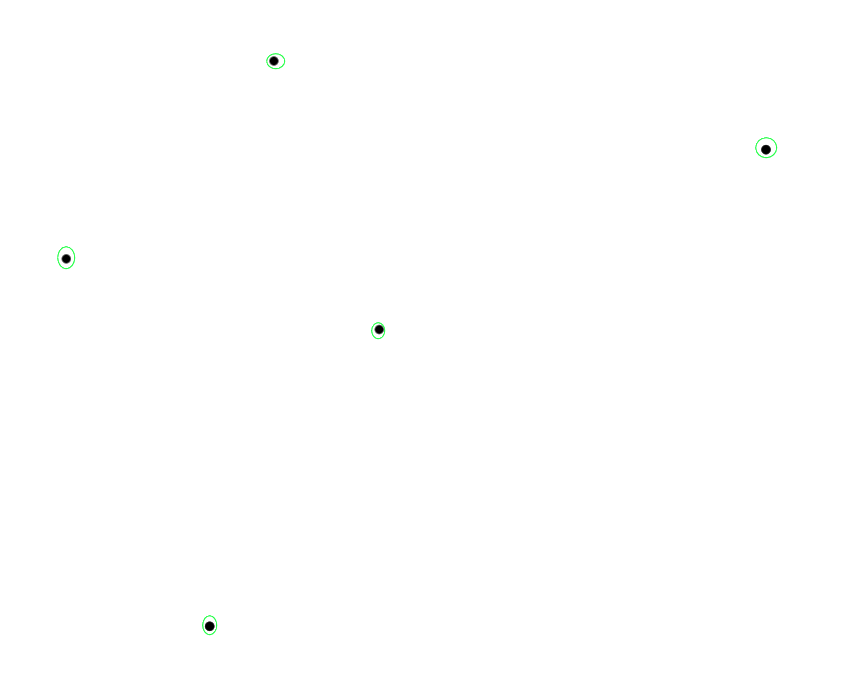
\includegraphics[width=9cm, height=6.5cm]{Term_3/Source/Pictures/voronoi0.png}
\end{center}
\end{frame}

\begin{frame}[fragile]{Наивный алгоритм}
\begin{center}
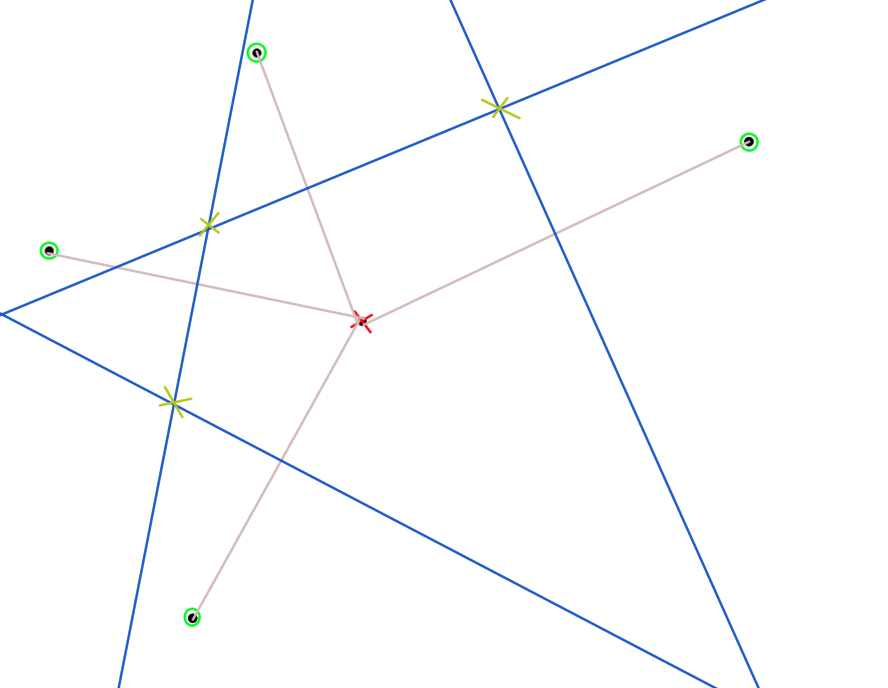
\includegraphics[width=9cm, height=6.5cm]{Term_3/Source/Pictures/voronoi1.png}
\end{center}
\end{frame}

\begin{frame}[fragile]{Наивный алгоритм}
\begin{center}
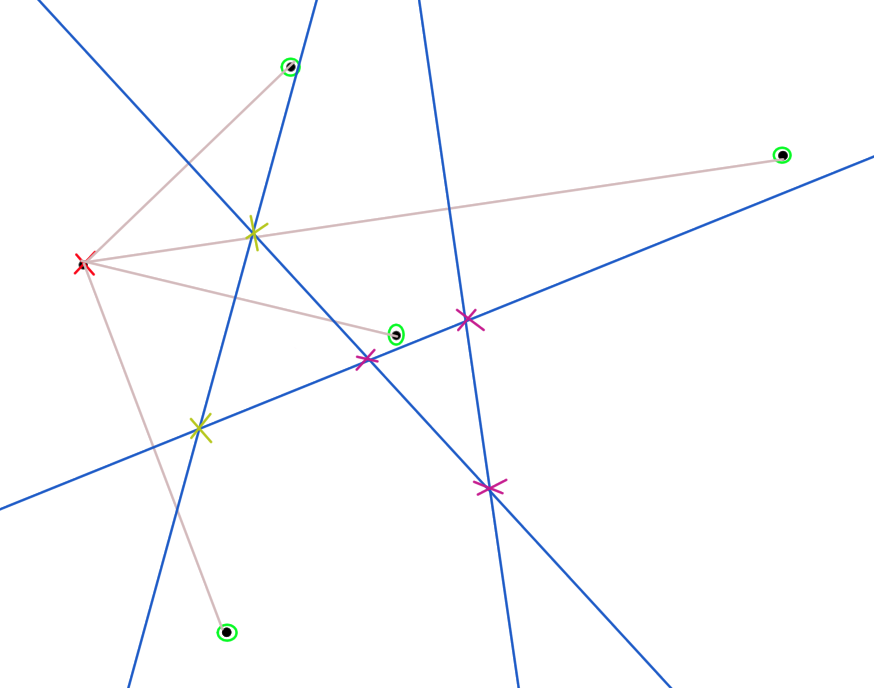
\includegraphics[width=9cm, height=6.5cm]{Term_3/Source/Pictures/voronoi2.png}
\end{center}
\end{frame}

\begin{frame}[fragile]{Наивный алгоритм}
\begin{center}
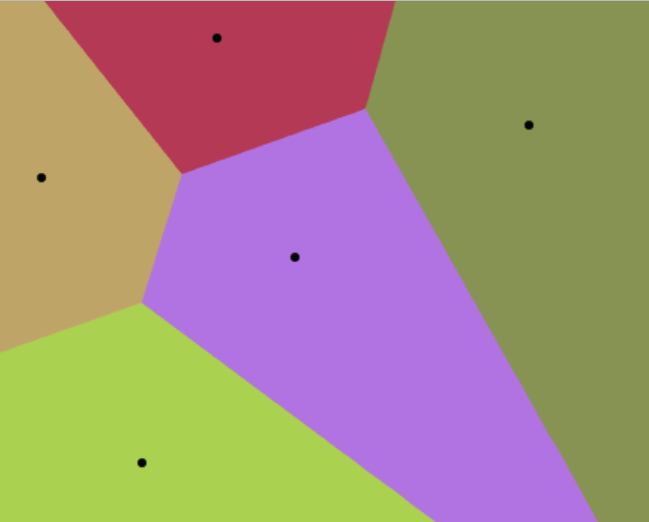
\includegraphics[width=9cm, height=6.5cm]{Term_3/Source/Pictures/voronoi3.png}
\end{center}
\end{frame}



\appendix
\section<presentation>*{\appendixname}
\subsection<presentation>*{Useful links}

\begin{frame}[allowframebreaks]
  \frametitle<presentation>{Полезные ссылки}
    
  \begin{thebibliography}{10}
{
  \beamertemplatebookbibitems
  \bibitem{interactive}
  \texttt{Interactive Voronoi Diagram Generator with WebGL}
  \newblock \href{http://alexbeutel.com/webgl/voronoi.html}{\texttt{http://alexbeutel.com/webgl/voronoi.html}}
  
  \bibitem{habr1}
  \texttt{Хабр: Диаграмма Вороного и её применения}
  \newblock \href{https://habr.com/post/309252/}{\texttt{https://habr.com/post/309252/}}
  
  \bibitem{habr2}
   \texttt{Хабр: рекурсивный алгоритм}
  \newblock \href{https://habr.com/post/314852/}{\texttt{https://habr.com/post/314852/}}
 
}
    
  \end{thebibliography}
\end{frame}

\end{document}


